% Source: Lecture2.pdf, pages 2-4 (page 1 is a stray cover image, not notes).
\lecture{2}
\subsubsection*{Liquid--gas and solid--liquid systems}

We continue the introduction to phase transitions with the solid--liquid--gas
(s--$\ell$--g) system. The order parameter is
\begin{equation}
  \Delta\rho = \rho_\ell - \rho_g \quad\text{or}\quad \rho_s-\rho_\ell .
\end{equation}

\begin{diagram}
\begin{tikzpicture}[scale=0.8,>=Stealth]
  \draw[->] (0,0) -- (5,0) node[below] {$T$};
  \draw[->] (0,0) -- (0,3.2) node[left] {$p$};
  \coordinate (tp) at (1.8,1.1); \coordinate (cp) at (3.6,2.4);
  \draw[thick] (0.4,0.2) .. controls (1,0.5) and (1.5,0.8) .. (tp);
  \draw[thick] (tp) .. controls (2.5,1.6) and (3.1,2.0) .. (cp);
  \draw[thick] (tp) .. controls (2,2) and (2.1,2.5) .. (2.2,3);
  \fill (tp) circle (0.05); \fill (cp) circle (0.05);
  \node at (0.9,1.8) {solid};
  \node[font=\small] at (2.5,2.3) {liq.};
  \node at (3.1,0.9) {gas};
  \node[anchor=west,font=\small] at (3.7,2.5) {critical pt.\ $(T_c,p_c)$};
\end{tikzpicture}
\diagramcaption{The solid--liquid--gas phase diagram.}
\end{diagram}

There are discontinuities across first-order phase boundaries, i.e.\ phase
coexistence curves. Consider heating a solid, e.g.\ H$_2$O:
\begin{equation}
  C_p = \left.\frac{\dd U}{\dd T}\right|_p ;
\end{equation}
we add heat energy and raise $T$, approaching $T_\ell$. For ice,
$C_p\sim 0.5\ \text{cal/g}$ (recall: $1\ \text{cal} = 4.186$~J).

Going from solid to liquid: at $T = T_\ell = 0^\circ$C we must add energy while $T$ is
unchanged. For H$_2$O,
\begin{equation}
  L_m = 79.7\ \frac{\text{cal}}{\text{g}} = 3.33\times 10^2\ \frac{\text{J}}{\text{g}}.
\end{equation}
Next, heat the liquid water, with $C_p$ = specific heat of liquid water
$= 1$~cal/g. Then, as the temperature reaches $T_v$ ($T_v = 100^\circ\text{C} = 373$~K
at $p = 1$~atm), again one must add $L_v$ = ``latent heat of vaporization'' to convert
the system from a liquid to a gas:
\begin{equation}
  L_v = 539\ \text{cal/g} = 2.26\times 10^3\ \text{J/g}.
\end{equation}
These values of $L_m$ and $L_v$ for water are larger than for other substances, e.g.\
for nitrogen, N$_2$:
\begin{equation}
  L_m = 6.1\ \text{cal/g},\quad T_m = 63.2\ \text{K at } p = 1\ \text{atm};\qquad
  L_v = 48\ \text{cal/g},\quad T_v = 77.3\ \text{K}.
\end{equation}

\subsubsection*{The critical point and critical singularities}

At the critical point there is a continuous phase transition (p.t.):
\begin{itemize}
  \item $G(T,p)$, liquid--gas system, at $p = p_c$, $T = T_c$;
  \item $G(T,H)$, magnetic system, at $H = H_c = 0$, $T = T_c$;
\end{itemize}
with nonanalytic behavior as a function of $T$ and the other variable ($p$ or $H$).
(Watch videos on pressure cells.)

Critical singularities:
\begin{itemize}
  \item specific heat:
  \begin{equation}
    C\sim
    \begin{cases}
      \tau^{-\alpha} & T\searrow T_c\\
      (-\tau)^{-\alpha'} & T\nearrow T_c
    \end{cases}
    \qquad\text{where}\quad \tau = \frac{T-T_c}{T_c}
  \end{equation}
  (some authors use $\epsilon\equiv\tau$);
  \item liquid--gas compressibility $\kappa = -(1/V)\left(\partial V/\partial p\right)_T$
    and magnetic susceptibility $\chi = \left(\partial M/\partial H\right)_T$:
  \begin{equation}
    \kappa,\ \chi\sim
    \begin{cases}
      \tau^{-\gamma} & T\searrow T_c\\
      (-\tau)^{-\gamma'} & T\nearrow T_c.
    \end{cases}
  \end{equation}
\end{itemize}

Order parameter: for a magnetic system, $M_{sp} = \lim_{H\to 0}M(H)$, with
\begin{equation}
  M_{sp}\sim(-\tau)^{\beta}\quad\text{as } \tau\to 0^-
\end{equation}
(don't confuse the critical exponent $\beta$ with $\beta = 1/(\kB T)$). For a
liquid--gas system, $\Delta\rho = \rho_\ell-\rho_g$ and
$\Delta\rho\sim(-\tau)^{\beta}$.

\begin{diagram}
\begin{tikzpicture}[scale=0.8]
  \draw (0,0) -- (4,0); \draw (0,0) -- (0,2.4);
  \node[left] at (0,1.6) {$M_{sp}$};
  \node[below] at (2.8,0) {$T_c$};
  \node[below] at (1,0) {$T$};
  \draw[thick] (0,2) .. controls (1.6,2) and (2.7,1.5) .. (2.8,0);
\end{tikzpicture}
\diagramcaption{The order parameter vanishes continuously as $T\to T_c^-$.}
\end{diagram}

\subsubsection*{Correlation functions and the correlation length}

A measure of ordering is the two-point correlation function:
\begin{align*}
  \text{liquid--gas:}&\quad\ev{\Delta\rho(\mathbf{x})\,\Delta\rho(\mathbf{y})}_{\text{conn}},\\
  \text{magnetic:}&\quad\ev{\mathbf{S}(\mathbf{x})\cdot\mathbf{S}(\mathbf{y})}_{\text{conn}}
  \quad\text{or Ising}\quad \ev{\sigma(\mathbf{x})\,\sigma(\mathbf{y})}_{\text{conn}},
\end{align*}
with asymptotic decay as $|\mathbf{x}-\mathbf{y}|\to\infty$
\begin{equation}
  \sim\exp\left[-|\mathbf{x}-\mathbf{y}|/\xi\right],\qquad \xi = \text{correlation length}.
\end{equation}
(There can be a power-law prefactor also.) The decay of short-range order at large
distance is characterized by the correlation length $\xi$. For $T\to\infty$, spins are
uncorrelated: $\ev{\sigma(\mathbf{x})\sigma(\mathbf{y})} = 0$ if $\mathbf{x}\ne\mathbf{y}$.
Now decrease $T$. As $T$ approaches $T_c$, the correlation length $\xi\to\infty$ in a
second-order phase transition. The critical singularity in $\xi$ is
\begin{equation}
  \xi\sim
  \begin{cases}
    \tau^{-\nu} & T\searrow T_c\\
    (-\tau)^{-\nu'} & T\nearrow T_c,
  \end{cases}
  \qquad \xi\to\infty\ \text{at } T_c.
\end{equation}
(In actual substances $\xi$ does not $\to\infty$, but is $\gg$ the interatomic spacing,
so approximately $\to\infty$.)

Definition: the connected two-point function is
\begin{equation}
  \ev{\mathbf{S}(\mathbf{x})\cdot\mathbf{S}(\mathbf{y})}_{\text{conn}}
  \equiv \ev{\mathbf{S}(\mathbf{x})\cdot\mathbf{S}(\mathbf{y})} - \ev{\mathbf{S}}^2 .
\end{equation}
This is the same as the full two-point function above $T_c$, where
$|\ev{\mathbf{S}}| = |\mathbf{M}_{sp}| = 0$.

\subsubsection*{Quantities at the critical point}

At $T_c$, along the ``critical isotherm'' for the order parameter,
\begin{equation}
  |\mathbf{M}(\mathbf{H})|\sim|\mathbf{H}|^{1/\delta},\qquad
  \Delta\rho\sim|p-p_c|^{1/\delta},
\end{equation}
and
\begin{equation}
  \left.
  \begin{array}{l}
    \ev{\mathbf{S}(\mathbf{x})\cdot\mathbf{S}(\mathbf{y})}\\[2pt]
    \ev{\sigma(\mathbf{x})\,\sigma(\mathbf{y})}
  \end{array}\right\}
  \sim\frac{1}{|\mathbf{x}-\mathbf{y}|^{d-2+\eta}},
\end{equation}
where $d$ = spatial dimensionality.

\begin{diagram}
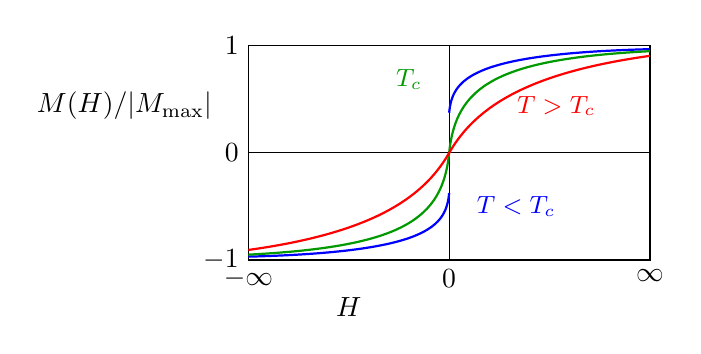
\begin{tikzpicture}[scale=0.85]
  \draw (0,0) rectangle (6,3.2);
  \draw (0,1.6) -- (6,1.6); \draw (3,0) -- (3,3.2);
  \node[below] at (0,0) {$-\infty$}; \node[below] at (3,0) {$0$}; \node[below] at (6,0) {$\infty$};
  \node[below=10pt] at (1.5,0) {$H$};
  \node[left] at (0,3.2) {$1$}; \node[left] at (0,1.6) {$0$}; \node[left] at (0,0) {$-1$};
  \node[left] at (-0.4,2.3) {$M(H)/|M_{\max}|$};
  \draw[thick,blue] (0,0.05) .. controls (2.7,0.12) and (2.95,0.5) .. (3,1.0);
  \draw[thick,blue] (3,2.2) .. controls (3.05,2.7) and (3.3,3.08) .. (6,3.15);
  \draw[thick,green!60!black] (0,0.08) .. controls (2.3,0.2) and (2.9,0.6) .. (3,1.6) .. controls (3.1,2.6) and (3.7,3.0) .. (6,3.12);
  \draw[thick,red] (0,0.15) .. controls (1.8,0.4) and (2.6,0.9) .. (3,1.6) .. controls (3.4,2.3) and (4.2,2.8) .. (6,3.05);
  \node[green!60!black,font=\small] at (2.4,2.7) {$T_c$};
  \node[red,font=\small] at (4.6,2.3) {$T>T_c$};
  \node[blue,font=\small] at (4,0.8) {$T<T_c$};
\end{tikzpicture}
\diagramcaption{Magnetization isotherms. For $T<T_c$ the magnetization jumps across
$H=0$; at $T=T_c$ it rises as $|H|^{1/\delta}$.}
\end{diagram}

Summary of critical exponents at a second-order phase transition:
$\{\alpha,\beta,\gamma,\nu\}$ and $\{\alpha',\gamma',\nu'\}$ for $T\ne T_c$,
$T\to T_c$; and $\{\delta,\eta\}$ at $T = T_c$.

\subsubsection*{Universality}

An important property of critical behavior and the associated critical exponents is
universality: they are independent of the details of the system, and only depend on
(1) the dimensionality $d$; (2) the symmetry group of the Hamiltonian.

Guggenheim, J.\ Chem.\ Phys.\ \textbf{13}, 253 (1945): data on the liquid--gas
transition in various substances (Ne, Ar, Kr, Xe, N$_2$, O$_2$, CO, CH$_4$),
\begin{equation}
  \Delta\rho = \rho_\ell-\rho_g\sim(-\tau)^{\beta}\quad\text{as }\tau\to 0^-,
\end{equation}
with measured value $\beta\sim1/3$ for all of these gases.

\begin{diagram}
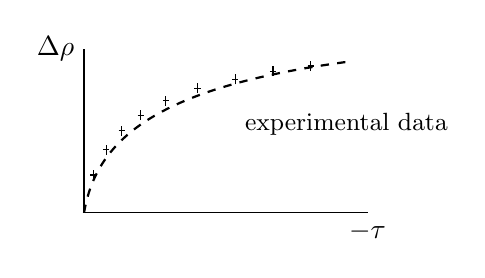
\begin{tikzpicture}[scale=0.8]
  \draw (0,0) -- (4.5,0) node[below] {$-\tau$};
  \draw (0,0) -- (0,2.6) node[left] {$\Delta\rho$};
  \draw[dashed,thick] (0,0) .. controls (0.2,1.2) and (1.2,2.0) .. (4.2,2.4);
  \foreach \x/\y in {0.15/0.6,0.35/1.0,0.6/1.3,0.9/1.55,1.3/1.78,1.8/1.98,2.4/2.12,3.0/2.25,3.6/2.33}
    \draw (\x-0.05,\y) -- (\x+0.05,\y) (\x,\y-0.08) -- (\x,\y+0.08);
  \node[anchor=west,font=\small] at (2.4,1.4) {experimental data};
\end{tikzpicture}
\diagramcaption{$\Delta\rho\sim(-\tau)^\beta$ fitted to liquid--gas data.}
\end{diagram}

E.g.\ Heller and Benedek (1962): similar universality was found in measurements of
$\beta$ for magnetic systems,
\begin{equation}
  M_{sp}\sim(-\tau)^{\beta}\quad\text{as }\tau\to 0^-
\end{equation}
(or $M_{\text{staggered}}$ for an antiferromagnet, $\uparrow\downarrow\uparrow\downarrow$),
so
\begin{equation}
  \ln M\sim\beta\ln(-\tau),\qquad \beta = \lim_{\tau\to 0^-}\frac{\ln M}{\ln(-\tau)}.
\end{equation}

\subsection{Physical scales and interatomic forces}
\subsubsection*{Sizes of relevant quantities}

Some sizes of relevant quantities in an atomic/molecular context, e.g.
\begin{equation}
  \hbar = 1.05\times 10^{-34}\ \text{J}\cdot\text{sec}
  = \frac{1.05\times 10^{-34}\ \text{J}\cdot\text{sec}}{1.60\times 10^{-19}\ \text{J/eV}}
  = 0.66\times 10^{-15}\ \text{eV-sec} = 0.66\ \text{eV-fs}
\end{equation}
($1\ \text{fs} = 10^{-15}$~sec). The value of $\hbar\sim(1\ \text{eV})(1\ \text{fs})\sim
\Order(1)$ in atomic-scale units.

For s--$\ell$--g phase transitions, $1\ \text{eV} = 1.60\times 10^{-19}$~Joules. The
product $\kB T$ is an energy; relate the MKS units to atomic/molecular units and
molecular bond strengths:
\begin{equation}
  \kB T = (1.38\times 10^{-23}\ \text{J/K})(1\ \text{K})
  = (0.862\times 10^{-4}\ \text{eV/particle})(1\ \text{Kelvin}).
\end{equation}
The bond strength for an ionic or covalent bond is
\begin{equation}
  \sim 100\ \text{kcal/mole} = \frac{(10^5)(4.186\ \text{J})}{(6.02\times 10^{23})(1.60\times 10^{-19}\ \text{J/eV})}
  = 4.35\ \text{eV/molecule}.
\end{equation}
N.B.: hydrogen bonds have strengths $\sim\Order(10)$ kcal/mol.

Pressure = force/area: $p = F/A = E/V$; the unit is Pa = N/m$^2$ (``Pascal''). Apply to
geophysics:
\begin{equation}
  (10\ \text{GPa})(10^{-10}\ \text{m})^3 = 10^{-20}\ \text{J}
  = \frac{10^{-20}\ \text{J}}{1.6\times 10^{-19}\ \text{J/eV}} = 6.3\times 10^{-2}\ \text{eV}.
\end{equation}

\begin{diagram}
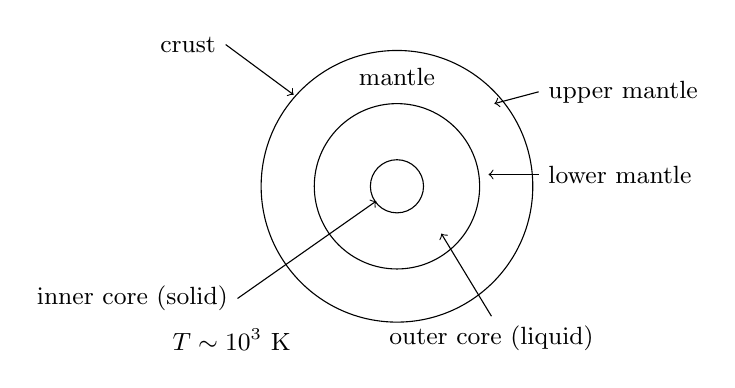
\begin{tikzpicture}[scale=0.75]
  \draw (0,0) circle (2.3);
  \draw (0,0) circle (1.4);
  \draw (0,0) circle (0.45);
  \draw[->] (-2.9,2.4) -- (-1.75,1.55); \node[anchor=east,font=\small] at (-2.9,2.4) {crust};
  \node[font=\small] at (0,1.85) {mantle};
  \draw[->] (2.4,1.6) -- (1.65,1.4); \node[anchor=west,font=\small] at (2.4,1.6) {upper mantle};
  \draw[->] (2.4,0.2) -- (1.55,0.2); \node[anchor=west,font=\small] at (2.4,0.2) {lower mantle};
  \draw[->] (-2.7,-1.9) -- (-0.35,-0.25); \node[anchor=east,font=\small] at (-2.7,-1.9) {inner core (solid)};
  \draw[->] (1.6,-2.2) -- (0.75,-0.8); \node[anchor=north,font=\small] at (1.6,-2.2) {outer core (liquid)};
  \node[font=\small] at (-2.8,-2.6) {$T\sim 10^3$ K};
\end{tikzpicture}
\diagramcaption{Layers of the earth.}
\end{diagram}

Here $1\ \text{atm} = 1\ \text{bar} = 100\ \text{kPa} = 0.1$~MPa. Typical values of
pressure in the earth (these pressures, and the associated temperatures, affect phase
changes in the rock):
\begin{itemize}
  \item $10$~kbar $= 1$~GPa: uppermost mantle;
  \item $\sim 100$~kbar $= 10$~GPa: upper mantle;
  \item $\sim 200$~kbar at the boundary between upper and lower mantle;
  \item $1.3$~Mbar $= 130$~GPa at the boundary between lower mantle and outer core;
  \item $3.3$~Mbar $= 330$~GPa at the boundary between outer (liquid) and inner (solid)
    core.
\end{itemize}
The phase transitions that occur in the rock in the interior of the earth involve
changes in crystal structure at high pressures and temperatures, i.e.\ solid--solid
phase transitions. At the boundary between the outer and inner core, there is a
liquid--solid phase transition. These properties were measured using seismology:
shear (transverse) waves travel through solids (at different speeds depending on
density), but not through liquid, while P (pressure, longitudinal) waves travel
through both solid and liquid.
